\documentclass[onecolumn, draftclsnofoot,10pt, compsoc]{IEEEtran}
\usepackage{graphicx}
\usepackage{url}
\graphicspath{ {./} }
%\usepackage{setspace}

\usepackage{geometry}
\geometry{textheight=9.5in, textwidth=7in}

\usepackage{hyperref}
\usepackage{listings}
%\usepackage{mdframed} %nice frames
\usepackage{xcolor} %custom colours
\definecolor{light-gray}{gray}{0.95}


% 1. Fill in these details
\def \CapstoneTeamName{			Addax}
\def \CapstoneTeamNumber{		38}
\def \GroupMemberOne{			Caitlyn Cook}
\def \GroupMemberTwo{			Iliana Javier}
\def \GroupMemberThree{			Nicholas Skinner}
\def \GroupMemberFour{			ChiaYu Tang}
\def \CapstoneProjectName{		Impala performance tuning on HDFS}
\def \CapstoneSponsorCompany{	HP Inc.}
\def \CapstoneSponsorPerson{	Andy Weiss}

% 2. Uncomment the appropriate line below so that the document type works
\def \DocType{	System Comparison	
	%Requirements Document
	%Technology Review
	%Design Document
	%Progress Report
}

\newcommand{\NameSigPair}[1]{\par
	\makebox[2.75in][r]{#1} \hfil 	\makebox[3.25in]{\makebox[2.25in]{\hrulefill} \hfill		\makebox[.75in]{\hrulefill}}
	\par\vspace{-12pt} \textit{\tiny\noindent
		\makebox[2.75in]{} \hfil		\makebox[3.25in]{\makebox[2.25in][r]{Signature} \hfill	\makebox[.75in][r]{Date}}}}
% 3. If the document is not to be signed, uncomment the RENEWcommand below
%\renewcommand{\NameSigPair}[1]{#1}

%%%%%%%%%%%%%%%%%%%%%%%%%%%%%%%%%%%%%%%
\begin{document}
	\begin{titlepage}
		\pagenumbering{gobble}
		%\begin{singlespace}s
		    	\includegraphics[height=4cm]{coe_v_spot1}
		\hfill 
		% 4. If you have a logo, use this includegraphics command to put it on the coversheet.
%	\includegraphics[height=4cm]{CompanyLogo}   
		\par\vspace{.2in}
		\centering
		\scshape{
			\huge CS Capstone \DocType \par
			{\large\today}\par
			\vspace{.5in}
			\textbf{\Huge\CapstoneProjectName}\par
			\vfill
			{\large Prepared for}\par
			\Huge \CapstoneSponsorCompany\par
			\vspace{5pt}
			{\Large\NameSigPair{\CapstoneSponsorPerson}\par}
			{\large Prepared by }\par
			Group\CapstoneTeamNumber\par
			% 5. comment out the line below this one if you do not wish to name your team
			\CapstoneTeamName\par 
			\vspace{5pt}
			{\Large
				\NameSigPair{\GroupMemberOne}\par
				\NameSigPair{\GroupMemberTwo}\par
				\NameSigPair{\GroupMemberThree}\par
				\NameSigPair{\GroupMemberFour}\par
			}
			\vspace{20pt}
		}
		\begin{abstract}
			% 6. Fill in your abstract    
The BackOffice team currently uses an Oracle database to store industrial IoT data gathered from large printing presses.
Due to a lapsing Oracle contract, there is an opportunity to move to a cheaper and more efficient option, with special interest in moving from the current “shared-everything” architecture to a “shared-nothing” architecture.
Based on their needs and available financial support, Cloudera’s Impala has been selected as the primary candidate for implementing the new system. 

In the first section of this report, we present our research on shared-everything architectures and their specific implementation in Oracle databases.
We also introduce shared-nothing architecture as a whole and its specific implementation in Cloudera Impala databases.
In the following sections, we provide specific details on the use of Impala including query coordination, explain plan, components of Impala server, SQL differences, query optimization and file formats.
 
In the Query Coordination section, we introduce how nodes take the role of query coordinator and assign work to other nodes once a query is sent.
We indicate that only one node runs certain Impala components, the \textit{statestored} and the \textit{catalogd}.
In the Explain Plan section, we provide examples of a Hue text based explain plan and a Hue visualized explain plan, to illustrate how each action would be executed step by step and provide guidance on how to read the plans.
The EXPLAIN command can help to level up the query and improve a user's understanding of the strategy taken by the compiler. 
The main components of an Impala system are described in the Impala Server Components section, including the statestore which communicates and checks the health of nodes, the catalog which manages metadata changes made by nodes, and the metastore, where all metadata is kept.

In the SQL Differences section, we discuss internal and external tables.
We also discuss partitioning in Impala, which is nested and created only for discrete values in specified partition columns.
The Query Optimization section describes several ways to make a query more efficient, including manipulating table statistics and SQL hints.
The Impala query planner stores detailed information of tables and partitions in metadata store with statistics.
SQL hints can be added as suggestions to improve the planner's decision-making. The SUMMARY and PROFILE statement can be used as monitoring tools to gain a better understanding of the execution, such as time used, memory usage and fragment information.
Lastly, we introduce Parquet, Avro and ORC, file formats that can be used in Hadoop clusters. Among them, only Parquet is in column-oriented file format and has the best performance in Impala. 

		\end{abstract}     
		%\end{singlespace}
	\end{titlepage}
	\newpage
	\pagenumbering{arabic}
	\tableofcontents
	% 7. uncomment this (if applicable). Consider adding a page break.
	%\listoffigures
	%\listoftables
	\clearpage
	
	% 8. now you write!
\section{Overview}
\subsection{Shared Everything}

\subsubsection{Concept}
In a shared everything environment, all servers and workload can access to the same shared store.
Meanwhile, they can read and write any portion of data they want easily.
In contrast to shared-nothing environment, the main feature is that clusters are able to exchange data with each other during computing.
This is one of the solutions for parallel database systems when processing huge data sets. 
To make clusters interactive, there are multiple ways of how clusters access data from each other.

\begin{figure}[ht]
    \begin{center}
    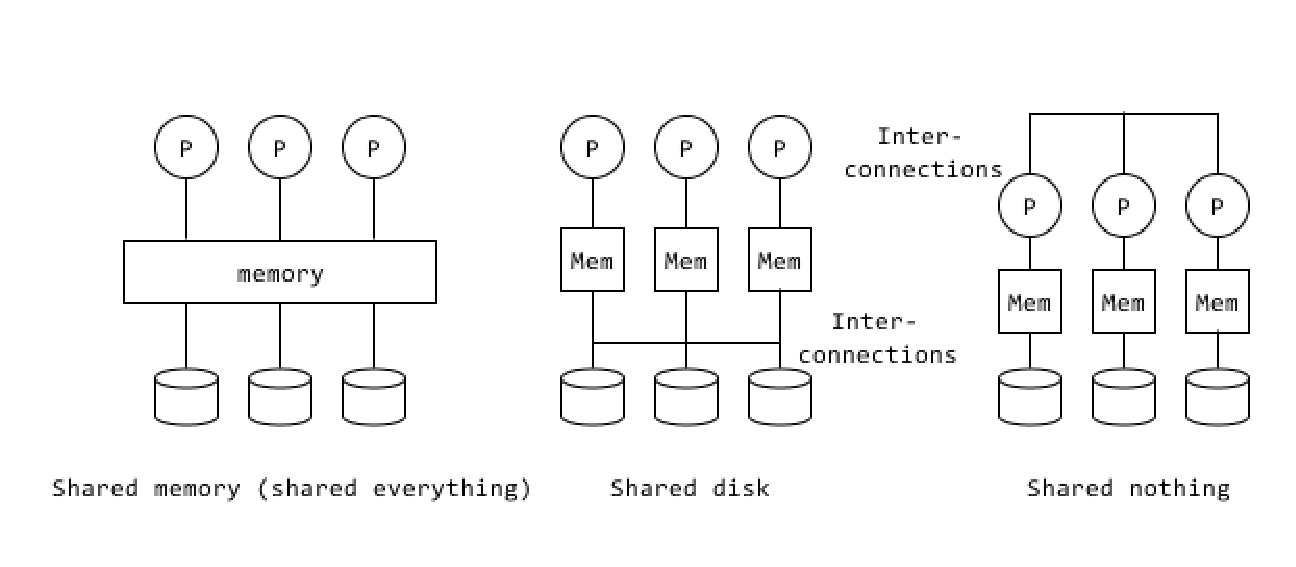
\includegraphics[height=2in, keepaspectratio]{amyImage1.eps}
    \caption{Architecture of Shared Memory System, Shared Disk System, and Shared Nothing System.}
    \end{center}
\end{figure}

Above, fig.1 is a basic diagram shows the different architecture between shared memory system and shared disk system. 
In shared memory system databases, each node or process is working with the same memory. 
If a node needs the calculation done by another node, it can access the updated data easily from the shared memory. 
In shared storage system, all connected systems share all storage disks. 
Each cluster still has it own local memory and can access to disks through interconnection.

Shared everything focuses on maximizing resource utilization \cite{ClaussenBestofBoth}. 
Since data may be cached in multiple places and accessed by any node in the system at any time, data consistency and contention may become an issue.
Although shared everything enables high scalability and performance, they are limited when lots of data are traveling through the interconnection at the same time. 
However, shared disk provides fault tolerant ability, which mean if one node fails then another node can complete the task as well.  

The choice of data structure is and important decision that influences the performance, stability and accessibility.
Tabular data are inherently rectangular.
More strictly, every row has the same set of column nodes and every record share same variables.
However, nested data are inherently in a tree layout.
This structure can be expected to faster than tabular since it enables processes to read less data.
Dremel and Solar are two successful distributed systems that implement shared everything architecture with nested data structure.
According to Dremel paper, it claims that nested data structure help their shared disk system access data faster and reduce CPU cost due to cheaper compression \cite{Dremel}.
On the other hand, Solar used the share everything architecture base on tree data set.
They increase the performance and scalability by adding storage nodes that are used for data storage and read access \cite{zhu2018solar}.  

Oracle is a shared everything database.
Specially, Oracle uses data dictionary to store their metadata. 
Data dictionary is formed with tables and views, and is being accessed frequently by the dictionary cache, where Oracle keeps data. 
The views in the data dictionary allows users to access and read data only.
The Oracle server accesses these two locations in order to share data for users access \cite{OracleDataDictionary}.
\subsubsection{Implementation}
Oracle is an example of a database system that implements the shared-everything model.
The data contained within the Oracle system is accessible to all the processing units without limitations \cite{OraclePEwODF}, meaning that the parallelism implemented within the Oracle system is not limited to the data access that an individual node would possess.
Rather, all dispatchable agents associated with the database are capable of accessing all the data contents.

Oracle’s shared-everything architecture does not require data partitioning to enable parallelism by default; data is accessible from all processing units without limitations \cite{OraclePEwODF}. 
Parallelism within the Oracle system is implemented through dividing a query into smaller components called granules.
Granules represent a fraction of a query, and can be assigned a specific block range in memory.
These block-based granules are assigned a position within the memory or the storage of the Oracle system, and will do all actions within their block range.
Partition-based granules leverage individual partitions of the database to further optimize query resolution speed.
Individual granules are capable of processing alongside other granules, enabling parallel execution throughout the system. 

Upon resolving a task, a granule will need to report its result set to another agent. 
The action it will take to complete this task is known as 'data redistribution', and it is a key component to many non-trivial parallel operations including parallel aggregations, joins and sorts \cite{OraclePEwODF}.
The individual granule does not know the broader context of the operation the retrieved data will be used within, so it must pass the result set to a subsequent operation on the result set contents.
The query coordinator will dispatch an agent to grab the result set from the previous granule, and assign the new agent a granule of work to process.
This series of events is recursively performed until the end query result is reached.

\begin{figure}[ht]
    \begin{center}
    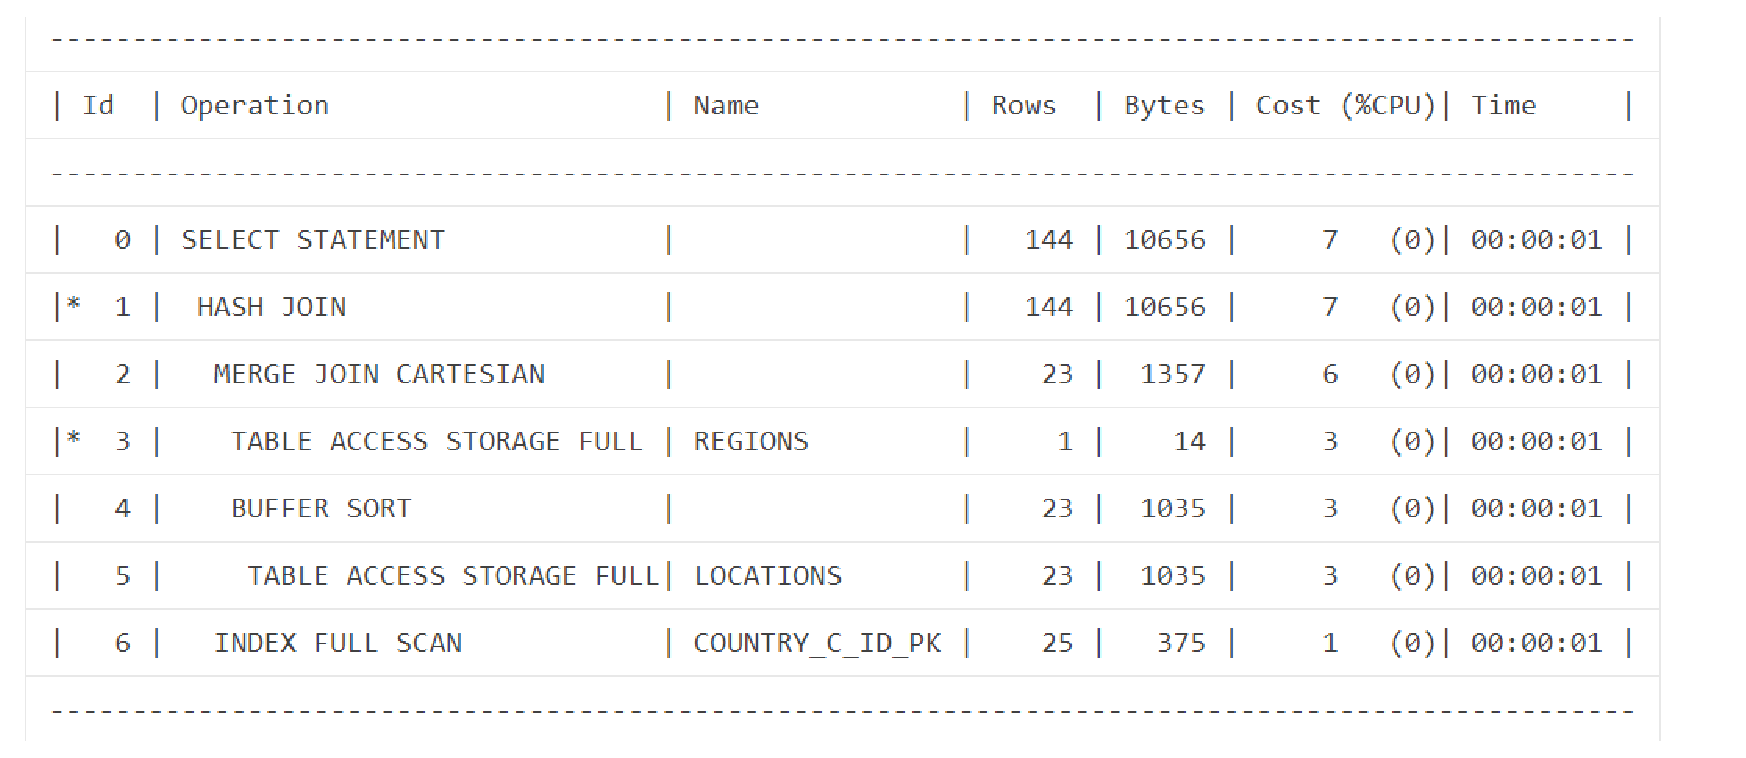
\includegraphics[width=6in, height=4in, keepaspectratio]{nickREimage.eps}
    \caption{Example of an explain plan as displayed in Oracle Live SQL using data from the HR schema.}
    \end{center}
\end{figure}

For further query optimization, Oracle is capable of operating on the same processing paradigm as a shared-nothing system.
If the Oracle partitioning feature is enabled, Oracle will assign each table a smaller result set, minimizing the amount of data that needs to be scanned. 
Oracle claims that the partitioning system carries the exact same parallel processing capabilities as a shared-nothing system, however, Oracle is capable of implementing this partitioning without the restrictions of the fixed parallel access encompassed in the data layout \cite{OraclePEwODF}.  

\subsection{Shared Nothing}
\subsubsection{Concept}
A shared nothing architecture is a model in which the processes do not share any resources. 
Each node within the system has its own memory and disk storage, rather than sharing one or both with other processes.
Each node would have a portion of the database’s stored data, and is the sole control on that portion of the data. 
The nodes connect through a network to coordinate actions by requesting information from each other. 

Shared nothing architectures are primarily used for their easy and relatively cheap scalability.
They can be built from commodity hardware, rather than requiring specialized and expensive parts to achieve high performance. 
One source estimated the cost of a single commodity node and a single specialized node at \$700 and \$10,000 \cite{HiPerf}. 
This source calculated that in order for specialized hardware to be as cost efficient, it must be at least 14 times as fast, which there is no indication of being true.

Shared nothing architectures are also not subject to the points of contention and bottlenecks that shared architectures have, such as the need for multiple nodes to read and write to the same data.
Rather than moving the data itself between processes, each node asks another node a question about the data it holds.
That node returns an answer which the asking node uses to continue with its work, until the complete question - the user’s query - is answered \cite{DeWittFuture}  .
This reduction in data transfer means that a higher proportion of time is spent processing the questions, which is a much easier task to speed up.
    
\subsubsection{Implementation}
Impala is an SQL engine that implements a shared-nothing, parallel processing architecture over Hadoop.
Queries are fragmented and distributed across nodes in the system to correspond with the portion of data stored locally on individual nodes.
The system was inspired by Google’s Dremel in that it uses columnar storage, executes SQL commands natively instead of building them on top of MapReduce jobs, and is specifically designed for distributed computing \cite{SQLonHadoop} \cite{Dremel}.
Impala takes it a step further and implements as pure of a shared-nothing architecture as it can.

An Impala system has three main components which work together to implement this shared-nothingness: the Impala daemon, the statestore daemon, and the catalog daemon. \cite{ImpalaGuide}. 
The \textit{impalad} is the Impala daemon which runs on every node in the system.
The responsibilities of an \textit{impalad} process include, but are not limited to: \cite{Impala} \cite{ImpalaGuide}
\begin{itemize}
    \item accepting initial queries
    \item reading and writing data files
    \item executing query fragments assigned to it
    \item transmitting intermediate query results back to the coordinator
\end{itemize} 
The coordinator is simply the first \textit{impalad} to receive an initial (raw SQL) query, at which point it assumes the coordinator role by managing that query’s execution across all other nodes and the assembly of the final query result \cite{Impala}. 
This avoids the need for a single node dedicated to coordinating all queries, since any \textit{impalad} in the system could be assigned the initial query.
Since an \textit{impalad} instance runs on every machine in the system, this allows Impala to take advantage of data locality, where each node can have its own partition of the data locally in own memory without having to use network communication to read other nodes’ data \cite{Impala}.

The \textit{statetored} further cements Impala as a shared-nothing system.
Each node working independently raises the issue of how coordinators can stay up to date on the other nodes in the system, and how they can be alerted if a node has failed.
An Impala cluster has a single daemon called a \textit{statestored} to push updates about the system to the nodes who need the information \cite{Impala}.
The \textit{statestored} maintains a table of topics, which is any information needed for query scheduling and execution \cite{ImpalaGuide}.
Processes running on nodes contact the \textit{statestored} only once, at startup, to give it a list of topics it needs to stay updated on \cite{Impala}. 
An important topic is the list of nodes in the system which are healthy and thus can accept work. 
For this topic, the \textit{statestored} monitors node health through the use of keepalive messages \cite{Impala}.
If a node goes offline (e.g. doesn’t respond to to the keepalive message), the \textit{statestored} broadcasts this change to the other \textit{impalad} processes, so they do not assign work to an unreachable node \cite{ImpalaGuide}.

The \textit{statestored} also broadcasts changes in metadata with help from the Catalog daemon.
Physically represented as the daemon process \textit{catalogd}, the catalog daemon pulls information from third-party metadata stores (e.g. the Hive Metastore or the HDFS Namenode), and aggregates that information into an Impala-compatible catalog structure \cite{Impala}. 
This is to make integration with third-party storage systems easier, while also allowing users to import Impala-specific information, such as user-defined functions \cite{Impala}.

\section{Query Coordination}
When a query is submitted to Impala, the node that receives it takes on the role of Query Coordinator (QC).
Any node can take on this role, and multiple nodes can be performing this role simultaneously for different queries.
Once a node takes on the role of QC for the query, it assigns work to known active nodes, including itself. 
All nodes complete their work on the data that they have, and return their results to the coordinating node, which compiles them and returns the information to the user. 

When possible, work is assigned so that data does not need to be transmitted from node to node.
Instead, the nodes holding that data are assigned the work needed to be done.
This improves execution time by taking advantage of data locality.
However, it is not always possible to execute in this way; for example, in the case of some joins, some table data must be transmitted between nodes. 

While it is a supposed advantage to distributed systems that there is no single point of failure since any node can become the coordinator, it is important to note that only one node runs \textit{statestored} and \textit{catalogd}.
Queries will not automatically fail should they be received while the node with these processes is down, but they will work with outdated information, which may have negative consequences. 
For more information on these processes, see the \hyperref[sec:impservcomp]{Impala Server Components} section.

\begin{figure}[ht]
    \begin{center}
    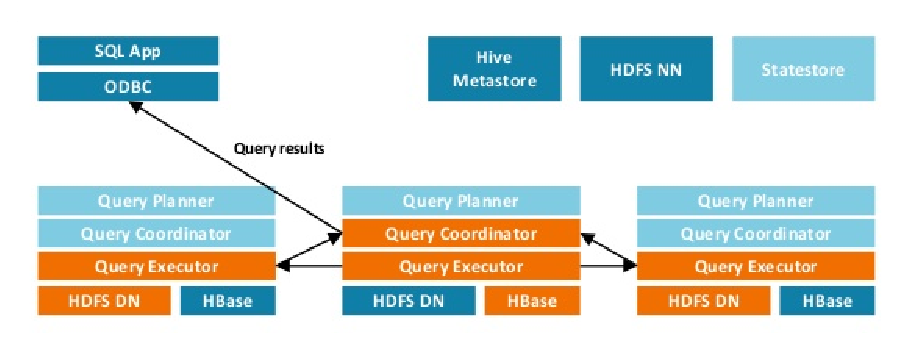
\includegraphics[width=4in, keepaspectratio]{qcc.eps}
    \caption{The flow of a query submitted to Impala. \cite{IncrImp}}
    \end{center}
\end{figure}

While the default behavior is for all nodes to act as both coordinator and executor when needed, it is possible to configure Impala with dedicated coordinator nodes.
This can reduce the amount of network traffic by reducing the amount of communication with the \textit{statestored} required, as only the coordinating nodes need to be aware of the status of all other nodes. 
This can be useful when there is a large volume of highly concurrent queries, which generate a large volume of traffic. 
If this option is chosen, it is recommended that there is about 1 dedicated coordinator for every 50 dedicated executors. 

\section{Explain Plans}
%introduce explain plans
%introduce how they display parallel execution
%
An explain plan in the Impala distributed system is a representation of how a query will be executed, or how it has been executed. The explain plan displays the Impala system's best estimate through incorporating Impala's current understanding of the environment around it. Statistics about performance and availability within the Impala system may influence how a plan will be generated, and what nodes it intends to seek out. 
%An explain plan in the Impala distributed system is a representation of how impala has, or how it intends to, resolve a selected query. 

%Parallel execution
When a query is executed, it may be divided into smaller tasks that may be executed in parallel.  
%explain levels
%level 0 is minimal
%level 1 is basic query summary
%level 2 includes hardware usage estimates
%level 3 is tuples and other info
To view an explain plan for a potential query, the query can be prepended with an EXPLAIN command. By default, he EXPLAIN command will display the current strategy the Impala system intends to attempt if it received the selected query. The EXPLAIN command can be set to be more verbose, causing it to include estimates on hardware usage, query breaking into nodes, and more items. The lower levels of usage can be obtained through setting the explain level to an appropriate level:
%\begin{mdframed}[backgroundcolor=light-gray, roundcorner=10pt,leftmargin=1, rightmargin=1, innerleftmargin=15, innertopmargin=10,innerbottommargin=10, outerlinewidth=1, linecolor=light-gray]
    \begin{center}
    \begin{lstlisting}[language=SQL]
set explain_level = 0; --Minimal - Displays tables and joins.
set explain_level = 1; --Standard - Default - Displays hashes and partitions.
set explain_level = 2; --Extended - How statistics were used in the planning.
set explain_level = 3; --Verbose - Shows how the query is broken into query 
                       --fragments within a node.
\end{lstlisting}
\end{center}
%\end{mdframed}
%explain plan after exec
To view an explain plan for a query that has already been resolved, use the PROFILE command. The PROFILE command will display a low-level query profile outline of the steps Impala took to resolve a query. The query profile will contain execution times for each step of query resolution to display possible bottlenecks encountered during execution. An ID for the query, as well as details about performance will also be included within the query profile.  
%introduce Hue visualization

Within the Hue editor, it is possible to display the explain plan in the query profile for any given query. When viewing the query details, it is possible to display an explain plan in a text based, and a visualized format. The following sections will display examples of both formats against the following query from the sample Oracle HR Schema:

%\begin{mdframed}[backgroundcolor=light-gray, roundcorner=10pt,leftmargin=1, rightmargin=1, innerleftmargin=15, innertopmargin=10,innerbottommargin=10, outerlinewidth=1, linecolor=light-gray]
    \begin{center}
    \begin{lstlisting}[language=SQL]
SELECT
       a.region_name,
       b.country_id,
       b.country_name,
       c.street_address,
       c.postal_code,
       c.city,
       c.state_province
FROM hr.regions a
INNER JOIN hr.countries b
    ON a.region_id = b.region_id
INNER JOIN hr.locations c
    ON b.country_id = b. country_id
WHERE a.region_name LIKE 'N%';
\end{lstlisting}
\end{center}
%\end{mdframed}

\subsection{Hue Text Based Explain Plan}
%content for explain plan
\begin{figure}[ht]
    \begin{center}
    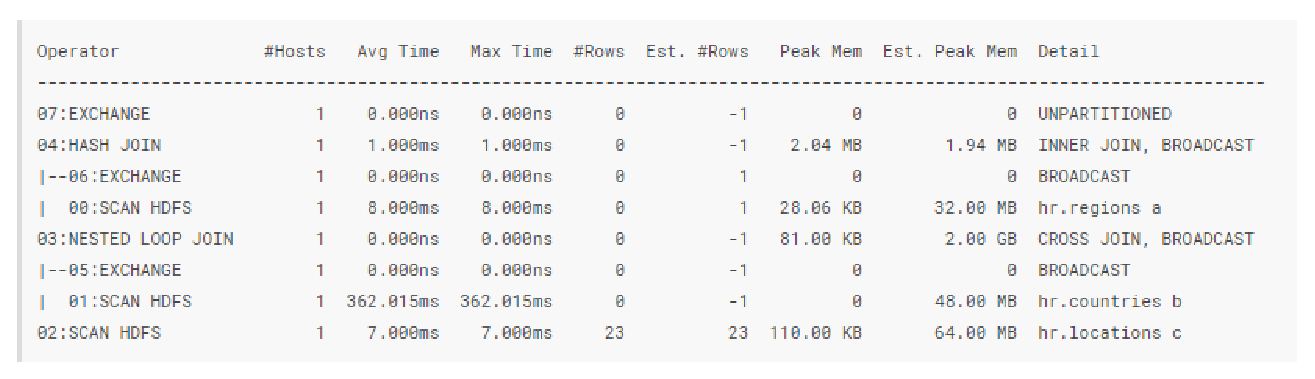
\includegraphics[width=6in, height=4in, keepaspectratio]{NickTextExplainPlan.eps}
    \caption{Example of a text explain plan as displayed in the Hue editor.}
    \end{center}
\end{figure}
%content for text explain plan
The text based explain plan is read from the bottom up, where indented items are portions of the query that are being executed in a separate branch parallel with the main query thread. Each action listed is one task that is assigned to one worker, similar to granules in the Oracle system. Reading the above figure, the first actions are scanning the hr.regions a table, and scanning the hr.countries b table. The next actions are to scan the hr.locations c table, broadcast the hr.locations b table results, and to scan for the hr.regions b table. Next, a join between the hr.countries b and the hr.locations c tables occurs while results from hr.regions a are broadcasted. When a result set is broadcasted, the contents from the resolved query fragment are sent to all other nodes involved in resolving the query. The joined tables hr.countries b and hr.locations c now join the broadcasted hr.regions a table, and an unpartitioned share is created. Impala broadcasts the final results to the client that sent the query through an unpartitioned share.
%should add a bit about hash joins
The text based explain plan also displays details relevant to the step of the query that it executed in a table format. Within the table, the number of rows that were retrieved during the specified phase of the query, the amount of time taken to execute individual steps, as well as the peak memory usage for those steps is displayed. This information may be used to reflect on performance of past queries, and guide planning of future query creation.
%pagebreak here because image was placing itself on next page without it
\pagebreak
\subsection{Hue Visualized Explain Plan}


%content for explain plan
\begin{figure}[ht]
    \begin{center}
    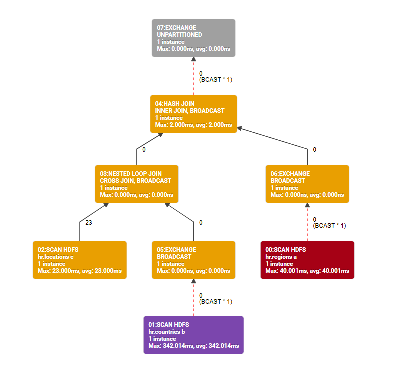
\includegraphics[width=6in, height=4in, keepaspectratio]{ExplainPlan.eps}
    \caption{Example of a visualized plan as displayed in the Hue editor.}
    \end{center}
\end{figure}


%content for explain plan
The visualized explain plan is read from the bottom to the top, where the bottom-most action represents the first action taken. Actions taken in parallel are represented on the same depth level. Each level also displays the number of results retrieved from its action, in the above example hr.locations c displays 23 along its flow line, indicating that it is sending 23 results to the next fragment of the query. Different colors represent different branches of the query, the branches may change color when combined with another branch of the query. In the above case, we have a separate color for when we retrieve the hr.countries b table, and another different color for hr.regions a. 

In the above figure, the first action is scanning the hr.countries b table. The next actions are to scan the hr.locations c table, broadcast the hr.locations b table results, and to scan for the hr.regions b table. Next, a join between the hr.countries b and the hr.locations c tables occurs while results from hr.regions a are broadcasted. The joined tables hr.countries b and hr.locations c now join the broadcasted hr.regions a table, and an unpartitioned share is created. 

\section{Impala Server Components}
\label{sec:impservcomp}
\subsection{The Impala Statestore}
The Impala statestore broadcasts service messages to each node in the cluster.
This is done to gain an understanding of the current state of the cluster, and any modifications that may need to be made.
The messages that are broadcasted come in two distinct forms: Heartbeats and Topic Updates.
These message types contain information the statestore requires to determine what actions it needs to take. 

A Heartbeat within the HDFS is an interaction between a datanode and its namenode intended to indicate presence.
The heartbeat exists as a keepalive message to ensure that the datanode is still working within the cluster.
After a user specified interval, if a number of heartbeats have not been received from the datanode, the namenode will consider the datanode to be out of service.
Blocks hosted by the out of service node will be marked as unavailable until the datanode is able to become active, or replicas of the available data blocks are created on other nodes.

A Topic Update within the HDFS is a message containing information on new developments regarding a topic.
The Topic update message will send and receive information from subscribers to specific topics.
An individual node is able to subscribe to modifications of topics of interest at start-up by providing a list of their topics of interest.
Subscribers of a specific topic will receive information on new entries, modified entries, and deletions.
If an individual node makes a change to a topic, it must wait for the statestored to broadcast a new topic update before other nodes are able to receive the new modifications. 

%Statestore Command Line Arguments:

The Impala statestore possesses command line arguments that may alter the number of process threads dedicated to its service as well as the frequency that update messages or heartbeats are sent to the associated nodes.
These arguments are to be appended to the command line startup.
A command to start the Impala statestore should look similar to the following statement:

%mdframed to make small light gray box around the code snippet.
%\begin{mdframed}[backgroundcolor=light-gray, roundcorner=10pt,leftmargin=1, rightmargin=1, innerleftmargin=15, innertopmargin=10,innerbottommargin=10, outerlinewidth=1, linecolor=light-gray]
    \begin{center}
    \begin{lstlisting}[language=bash]
$ sudo service impala-state-store start
    \end{lstlisting}
    \end{center}
%\end{mdframed} 

If a restart is required, the following command should be used:
%\begin{mdframed}[backgroundcolor=light-gray, roundcorner=10pt,leftmargin=1, rightmargin=1, innerleftmargin=15, innertopmargin=10,innerbottommargin=10, outerlinewidth=1, linecolor=light-gray]
    \begin{center}
    \begin{lstlisting}[language=bash]
$ sudo service impala-state-store restart
    \end{lstlisting}
    \end{center}
%\end{mdframed}

%number of threads
The following command will modify the current number of threads that are dedicated to sending topic updates. Official Impala documentation suggests to keep this at its default value of 10.
%\begin{mdframed}[backgroundcolor=light-gray, roundcorner=10pt,leftmargin=1, rightmargin=1, innerleftmargin=15, innertopmargin=10,innerbottommargin=10, outerlinewidth=1, linecolor=light-gray]
    \begin{center}
    \begin{lstlisting}[language=bash]
-statestore_num_update_threads 10
    \end{lstlisting}
    \end{center}
%\end{mdframed}

%Statestore Update Frequency
This command will set the frequency, designated in milliseconds, that the statestore attempts to send a Topic Update to each subscriber. By default Topic Updates occur every 2000 milliseconds (every 2 seconds).
%\begin{mdframed}[backgroundcolor=light-gray, roundcorner=10pt,leftmargin=1, rightmargin=1, innerleftmargin=15, innertopmargin=10,innerbottommargin=10, outerlinewidth=1, linecolor=light-gray]
    \begin{center}
    \begin{lstlisting}[language=bash]
-statestore_update_frequency_ms 2000
    \end{lstlisting}
    \end{center}
%\end{mdframed}

%Heartbeat Number of Threads
The following command will modify the current number of threads that are dedicated to sending heartbeats. Official Impala documentation suggests to keep this at its default value of 10.
%\begin{mdframed}[backgroundcolor=light-gray, roundcorner=10pt,leftmargin=1, rightmargin=1, innerleftmargin=15, innertopmargin=10,innerbottommargin=10, outerlinewidth=1, linecolor=light-gray]
    \begin{center}
    \begin{lstlisting}[language=bash]
-statestore_num_heartbeat_threads 10
    \end{lstlisting}
    \end{center}
%\end{mdframed}

%Heartbeat frequency
This command will set the frequency, designated in milliseconds, that the Statestore attempts to send a heartbeat to each subscriber. By default heartbeat messages occur every 1000 milliseconds (every 1 second). Impala claims that this value should be capable of supporting catalogs and clusters up to 150 nodes, beyond that you may be required to increase the heartbeat delay.

%\begin{mdframed}[backgroundcolor=light-gray, roundcorner=10pt,leftmargin=1, rightmargin=1, innerleftmargin=15, innertopmargin=10,innerbottommargin=10, outerlinewidth=1, linecolor=light-gray]
    \begin{center}
    \begin{lstlisting}[language=bash]
-statestore_heartbeat_frequency_ms 1000
    \end{lstlisting}
    \end{center}
%\end{mdframed}

    
\subsection{The Impala Catalog Service}
The Impala Catalog Service is a component of the Impala server that relays metadata changes from Impala DDL and DML statements.
This catalog service is physically represented by a daemon process \textit{catalogd} which interfaces with the statestore component to collect metadata changes for each Impala node. % TODO Investigate better emphasis
Metadata changes are then collected into a unified database named the ‘Metastore’, which is intended to create a metadata directory to assist query resolution speeds.
The Impala Catalog Service exists to minimize need for manual refreshes of metadata store (The SQL commands REFRESH and INVALIDATE METADATA are still valid if not changing any DDL/DML directly).
Updates to the metastore performed by the catalogd daemon are performed every topic update. 

Even with automatic metastore updates, the Impala Catalog Service is unable to detect new information and modifications to the dataset from specific methods of interfacing with the Impala ecosystem.
The following actions will not cause a Metastore update:

\begin{itemize}
    \item DDL/DML statements done through HIVE
    \item Manipulating data files directly within the HDFS
    \item Any non-DDL/DML statement changes to the dataset
\end{itemize}

In these instances, the Catalog Service is unable to detect changes within the system, and is unable to force a refresh on the Metastore. To resolve this, a manual refresh command must be executed against at least one node.

Because requests by the catalogd daemon are passed through the statestore daemon, it is recommended to run both services on the same host. This will reduce the network communication required between the systems.

The catalogd daemon is a non-critical service, meaning it does not need to be active at all times. When an error prevents the catalogd service from carrying an action, no data loss occurs, though the metastore may not possess the latest metadata from each node. If the daemon has not been run for an extended period, and a REFRESH command has not been executed, the data possessed by the metastore will be out of date, but is still accessible by virtue of being hosted through the statestore.

The catalog daemon comes with a select few arguments that can control how the service loads metadata.
The service itself can be started by issuing the host machine the following command:
%\begin{mdframed}[backgroundcolor=light-gray, roundcorner=10pt,leftmargin=1, rightmargin=1, innerleftmargin=15, innertopmargin=10,innerbottommargin=10, outerlinewidth=1, linecolor=light-gray]
    \begin{center}
    \begin{lstlisting}[language=bash]
$ sudo service impala-catalog start
    \end{lstlisting}
    \end{center}
%\end{mdframed}

If a restart is required, the user is able to simply use the following command:
%\begin{mdframed}[backgroundcolor=light-gray, roundcorner=10pt,leftmargin=1, rightmargin=1, innerleftmargin=15, innertopmargin=10,innerbottommargin=10, outerlinewidth=1, linecolor=light-gray]
    \begin{center}
        \begin{lstlisting}[language=bash]
$ sudo service impala-catalog restart
        \end{lstlisting}
    \end{center}
%\end{mdframed}

The Catalog Service provides an argument option to either load all metadata before accepting a request, or asynchronously load data to enable sending requests as soon as the service is started.
Asynchronous loading is the current default option in Impala, however, the other method can be enacted through the following argument:
%\begin{mdframed}[backgroundcolor=light-gray, roundcorner=10pt,leftmargin=1, rightmargin=1, innerleftmargin=15, innertopmargin=10,innerbottommargin=10, outerlinewidth=1, linecolor=light-gray]
    \begin{center}
\begin{lstlisting}[language=bash]
--load_catalog_in_background=false
\end{lstlisting}
\end{center}
%\end{mdframed}

\subsection{The Metastore}
Impala keeps table definitions for each node within a centralized traditional database called the metastore. 
Impala also tracks additional metadata for the low-level characteristics of data files, including the physical locations of blocks within HDFS. 
Each Impala node caches all of this metadata to reuse for future queries against the same table. 
The metastore collects metadata from each node in a cluster, and shares this collected data with all the nodes in the cluster.

Metadata within the HDFS is capable of being automatically updated through the catalogd daemon if the modifications are limited to a DDL or a DML change. 
The catalogd daemon relays the metadata changes from Impala SQL statements to all the Impala daemons in a cluster. 
For more information about the catalogd daemon, refer to the Impala Catalog Service section. 
 
When needed, a manual metadata refresh can be performed by executing either the INVALIDATE METADATA or the REFRESH commands on a specified table. 
INVALIDATE METADATA [table\_name] will reload all metadata for the specified table, updating all facets of the system’s understanding of the current metadata composition.
The REFRESH [table\_name] command will only update the metadata of the table with the locations of newly added blocks.
REFRESH allows a lightweight update of the system, but if more extensive changes have been made, it is recommended to use INVALIDATE METADATA to avoid performance degradation.
If a metadata update of the entire system is required, it can be performed by using INVALIDATE METADATA with no table suffix, this will cause the Impala system to tag each node to re-create metadata for all tables.
    
\section{SQL Differences}
    \subsection{Table Creation}
        \subsubsection{Internal and External Tables}
To create a table, use the CREATE TABLE statement.
By default, an internal table is created; an external table can be created by adding EXTERNAL to the statement. 

When an internal table is created, Impala creates the necessary directory to hold the data in the default Impala workspace.
Data is then added to the table after creation using the INSERT or LOAD DATA statements.
If the table is renamed, Impala will move the files to a directory with the new name, even if the files were originally located outside of its workspace.
If the table is dropped, Impala will delete all data files in the table. 

By contrast, an external table’s files are not directly managed by Impala.
When creating an external table you should supply a LOCATION statement that tells Impala where the files are stored. 
If you do not supply a location, Impala will use the default location, as if it were an internal table, but will still not manage the files. 
Impala will treat any files in this location as part of the table, and new data can be added through INSERT or LOAD DATA statements as with internal tables. 
If the table is renamed or dropped, Impala will not modify the files at all, since it is not managing them. 
Dropping the table will remove Impala’s association with it, but they may continue to be used by other Hadoop or HDFS components. 
Otherwise, an external is the same as an internal table. It can contain any file type, and will behave the same as an internal table.

Alternatively to creating a table and loading/inserting data, you can use a CREATE TABLE AS SELECT statement.
In this case, omit the column definitions at the top of the statement, and add a SELECT statement beneath all options. 
You may also choose to omit column definitions if you are loading a Parquet file, as they may be inferred from the file itself.
In this case, provide a LIKE PARQUET \textless path\_to\_file\textgreater  statement where the column definitions would otherwise go.

\begin{figure}[ht]
    \begin{center}
        
    \begin{lstlisting}[language=SQL]
CREATE [EXTERNAL] TABLE [IF NOT EXISTS] [db_name.]table_name
    (col_name data_type [COMMENT 'col_comment'] 
    [, ...])
    [PARTITIONED BY (col_name data_type [COMMENT 'col_comment'], ...)]
    [SORT BY ([column [, column ...]])]
    [COMMENT 'table_comment']
    [ROW FORMAT row_format]
    [WITH SERDEPROPERTIES ('key1'='value1', 'key2'='value2', ...)]
    [STORED AS file_format]
    [LOCATION 'hdfs_path']
    [CACHED IN 'pool_name' [WITH REPLICATION = integer] | UNCACHED]
    [TBLPROPERTIES ('key1'='value1', 'key2'='value2', ...)]
\end{lstlisting}
    \caption{Syntax for creating a table}
    \end{center}

\end{figure}

\begin{figure}[ht]
    \begin{center}
    \begin{lstlisting}[language=SQL]
CREATE [EXTERNAL] TABLE [IF NOT EXISTS] db_name.]table_name
    [PARTITIONED BY (col_name[, ...])]
    [SORT BY ([column [, column ...]])]
    [COMMENT 'table_comment']
+   [ROW FORMAT row_format]
    [WITH SERDEPROPERTIES ('key1'='value1', 'key2'='value2', ...)]
+   [STORED AS ctas_file_format]
    [LOCATION 'hdfs_path']
+   [CACHED IN 'pool_name' [WITH REPLICATION = integer] | UNCACHED]
    [TBLPROPERTIES ('key1'='value1', 'key2'='value2', ...)]
 AS
    <select_statement>
\end{lstlisting}
    \caption{Syntax for creating a table as select}
    \end{center}
\end{figure}

        \subsubsection{Partitioning}
Unlike Oracle, there is only one kind of partitioning in Impala.
Partitions are created for discrete values in specified partition columns. 
You cannot specify ranges or hashes to partition on. 
If you would like to partition by one of these methods, you should create a column in the table such that each desired range or hash value is represented as a distinct value in the column (i.e. Jan 1 - 31 is rangecol=1, Feb 1 - 28 is rangecol=2, etc). 

Partitioning is represented in the files as a nested directory structure. 
Each value of the partition is a directory, which may contain more directories as additional partitions or data files at the lowest level of partitioning. 
Indexes are not supported in Impala; however, the nested structure of partitions means that they can simulate some of the performance gains of the index.

Partitions are defined in the CREATE statement for the table. 
Once the table and its partitions have been created, it is not possible to add new data to existing partitions. 
It is possible, however, to add new partitions entirely (ie adding a new year to a table partitioned by year).
If it is necessary to modify an existing partition, you must remove and recreate the partition with your changes added. 

When partitioning on time values, you should separate the times you want to partition on as discussed above.
Because Impala partitions on discrete values of a column and not ranges, it cannot partition directly on a TIMESTAMP; doing so would specify a partition for each microsecond, and have no more than one value in each partition.

    \subsection{Analytic Functions}
The following analytic and aggregate functions are supported by Impala:
\begin{center}
\begin{tabular}{ |c|c| }
    \hline
    Analytic & Aggregate \\
    \hline
    AVG & APPX\_MEDIAN \\
    COUNT & AVG \\
    CUME\_DIST & COUNT \\
    DENSE\_RANK & GROUP\_CONCAT \\
    FIRST\_VALUE & MAX \\
    LAG & MIN \\
    LAST\_VALUE & NDV \\
    LEAD & STDDEV,  \\
    MAX & STDDEV\_SAMP \\
    MIN & STDDEV\_POP \\
    NTILE & SUM \\
    PERCENT\_RANK & VARIANCE \\
    ROW\_NUMBER & VARIANCE\_SAMP\\
    SUM & VAR\_POP \\
    \hline
\end{tabular}
\end{center}
The AVG, COUNT, MAX, MIN, and SUM functions can be used as either analytic or aggregate functions. 
When these functions are provided an ORDER\_BY clause, they operate as analytic functions.
If an ORDER\_BY clause is not supplied, they operate as aggregate functions. 

The value of analytic functions is calculated for each row depending on the window of rows specified, and returned with the results of that row.
If a windowing clause is not explicitly supplied, the assumed window is RANGE BETWEEN UNBOUNDED PRECEDING AND CURRENT ROW; that is, the current row and all rows before it.
This is the same default behavior as in Oracle. 

In Impala, it is not possible to select a window of a variable size using the RANGE BETWEEN statement. 
You may only select unbounded either preceding, following, or both. 
It is not possible to range between a specific value such as time, for example. 
You may select a specific number of rows using the ROWS BETWEEN, for example to calculate a moving average.

\begin{figure}[ht]
    \begin{center}
    \begin{lstlisting}
function(args) OVER([partition_by_clause] [order_by_clause [window_clause]])

partition_by_clause ::= PARTITION BY expr [, expr ...]
order_by_clause ::= ORDER BY expr  [ASC | DESC] [NULLS FIRST | NULLS LAST] 
                                   [, expr [ASC | DESC] [NULLS FIRST | NULLS LAST] ...]

window_clause ::= { ROWS BETWEEN  [ { m | UNBOUNDED } PRECEDING | CURRENT ROW] 
                                  [ AND [CURRENT ROW | { UNBOUNDED | n } FOLLOWING] ]
                  | RANGE BETWEEN [ {m | UNBOUNDED } PRECEDING | CURRENT ROW] 
                                  [ AND [CURRENT ROW | { UNBOUNDED | n } FOLLOWING] ] }
\end{lstlisting}
    \caption{Use and definition of analytic function clauses}
    \end{center}
\end{figure}
    
\section{Query Optimization}
The Impala query planner chooses optimizations based on the available table and column statistics.
A heavy emphasis is placed on the size and number of rows that will be involved at each stage of processing, as well as how data is distributed across nodes.
Impala uses this information to help parallelize and distribute the work for a query in the most efficient manner calculated by the query optimizer.

Query optimizations can also be influenced manually by manipulating table statistics and by including SQL hints in the query itself.

\subsection{Statistics}
The Impala query planner can use statistics about entire tables as well as individual partitions in its decision process.
These statistics are stored in the metadata store.
(See The Impala Catalog Service section for more details about the metadata store.)  

To calculate statistics for a given table, run the COMPUTE STATS command. 
Computed statistics can be viewed using the SHOW TABLE STATS command:

% TODO Code snippet
%\begin{mdframed}[backgroundcolor=light-gray, roundcorner=10pt,leftmargin=1, rightmargin=1, innerleftmargin=15, innertopmargin=10,innerbottommargin=10, outerlinewidth=1, linecolor=light-gray]
    \begin{center}
    \begin{lstlisting}[language=SQL]
COMPUTE STATS table_name;
SHOW TABLE STATS table_name;
\end{lstlisting}
\end{center}
%\end{mdframed}

For unpartitioned tables, SHOW TABLE STATS results in a single row summarizing the entire table, with columns representing the number of rows, number of files, size, bytes cached, cache replication, file format, if incremental statistics are available (covered later in this section), and the physical location of the table in memory. 
In partitioned tables, this results in a similar table, except each row now represents a different partition. 
Columns in this table represent the number of rows, number of files, etc for each particular partition. 
The final row in this table represents the total table statistics, as if the table were unpartitioned. 
If a statistic has not been calculated or is unavailable, the value -1 is used as a placeholder.

In addition to whole table statistics, statistics gathered on a by-column basis are also useful for query optimization. This technique is most useful when comparing columns across tables in JOIN queries, this helps estimate the number of rows the query will need to get from each table.
The COMPUTE STATS command computes column statistics as well as full table statistics.
Column statistics can be seen using the SHOW COLUMN STATS command. 

%\begin{mdframed}[backgroundcolor=light-gray, roundcorner=10pt,leftmargin=1, rightmargin=1, innerleftmargin=15, innertopmargin=10,innerbottommargin=10, outerlinewidth=1, linecolor=light-gray]
    \begin{center}
    \begin{lstlisting}[language=SQL]
SHOW COLUMN STATS table_name;
\end{lstlisting}
\end{center}
%\end{mdframed}

Unlike table statistics, partitioning does not affect column statistic gathering, because column statistics are only calculated for the entire table, not individual partitions.
However, an additional kind of statistics, called Incremental Statistics, can be gathered for partitioned tables. 

When you compute incremental statistics, statistics are only gathered for partitions that do not yet have incremental statistics. This way, statistics are only computed for newly added partitions, instead of for the entire table. This keeps statistics up to date without incurring the overhead of reprocessing the entire table each time data is added. They can be computed with the command:

%\begin{mdframed}[backgroundcolor=light-gray, roundcorner=10pt,leftmargin=1, rightmargin=1, innerleftmargin=15, innertopmargin=10,innerbottommargin=10, outerlinewidth=1, linecolor=light-gray]
    \begin{center}
    \begin{lstlisting}[language=SQL]
COMPUTE INCREMENTAL STATS table_name [partition_key];
\end{lstlisting}
\end{center}
%\end{mdframed}

Running the above command without a specified partition causes incremental stats to be computed for all partitions currently without incremental stats.
If it is the first time is it run, it will compute stats for the whole table. 
However, all future runs will only compute stats for new partitions.
Due to this, computing incremental stats will take more time than the regular COMPUTE STATS command for the same volume of data, and so should not be used for regularly updating entire tables worth of statistics. 
Computing incremental stats also uses some memory in the \textit{catalogd} process -- about 400 bytes of overhead memory for each column in a partition.

To maintain accurate statistics for each table, run your chosen COMPUTE STATS command every time new data is loaded into a table, and after the amount of data in a table is changed significantly, such as from an INSERT, add PARTITION, or LOAD DATA command. 

\subsection{Manual Statistic Manipulation}
There are many cases where manually manipulating table and column statistics is useful, including but not limited to:
\begin{itemize}
    \item When running a full COMPUTE STATS command is not time efficient
    \item When the current metadata causes the Impala optimizer to choose an inefficient JOIN operation
    \item When adding data to a table which has less columns than the data 
    \item When importing a new table with which you wish to use the statistics of an existing table instead of computing new statistics
\end{itemize}

In such cases, the metadata where table statistics are stored can be changed using an ALTER TABLE command. 

The most useful metadata to change will be the number of rows contained in a table. 
You can change the number of rows by table and by partition.
In the below example, we first set a table named table\_name’s number of rows to be 100, then we set a specific partition of table\_name, partitionP (partitioned based on ‘year’ and ‘month’) , number of rows to be 5. 
Remember, the ALTER TABLE command does not change the actual data,  just the metadata store. 
The data file table\_name is stored in will still have its original number of rows after the command is run.

%\begin{mdframed}[backgroundcolor=light-gray, roundcorner=10pt,leftmargin=1, rightmargin=1, innerleftmargin=15, innertopmargin=10,innerbottommargin=10, outerlinewidth=1, linecolor=light-gray]
    \begin{center}
    \begin{lstlisting}[language=SQL]
-- change the numRows property for whole table
ALTER TABLE table_name SET tblproperties( 'numRows' = '100', 
                                          'STATS_GENERATED_VIA_STATS_TASK'='true');
                                           
-- change the numRows property for the partition
ALTER TABLE table_name partition(year=2009, month=4)
SET tblproperties ('numRows'='5', 'STATS_GENERATED_VIA_STATS_TASK'='true'); 
\end{lstlisting}
\end{center}
%\end{mdframed}

In CDH 5.8 / Impala 2.6 and higher, you can append commands to ALTER TABLE to manipulate the statistic values of a specific column.
You can only set statistic values for the entire table’s columns.
As of the writing of this paper, you cannot set column statistics by partition.
You also can only alter statistic values for one column per command.
If you wish to set statistics for multiple columns, this must be done in separate commands.

Changing statistics requires use of case-insensitive symbolic names for each statistics:
\begin{center}
\begin{tabular}{ |c|c| }
    \hline
    Statistic Name & Symbolic Name \\
    \hline
    Number of Distinct Values  & numDVs \\
    Number of Null Values & numNulls \\
    Average Size of Data & avgSize \\
    Maximum Size of Data & maxSize \\
    \hline
\end{tabular}
\end{center}

To change these statistics using the SET COLUMN STATS command, both the symbolic (key) names and their new values must be quoted as in the examples below.

%\begin{mdframed}[backgroundcolor=light-gray, roundcorner=10pt,leftmargin=1, rightmargin=1, innerleftmargin=15, innertopmargin=10,innerbottommargin=10, outerlinewidth=1, linecolor=light-gray]
    \begin{center}
    \begin{lstlisting}[language=SQL]
-- alter column1's number of distinct values and number of nulls
ALTER TABLE table_name 
SET COLUMN STATS col_name1('numDVs'='2','numNulls'='0'); 

--alter column2's number of distinct values and max size 
ALTER TABLE table_name 
SET COLUMN STATS col_name2 ('numDVs'='3','maxsize'='4');
\end{lstlisting}
\end{center}
%\end{mdframed}

A key demonstration of how ALTER TABLE does not affect the underlying data files is by observing the ADD COLUMNS and DELETE COLUMN commands.
Adding column metadata via ALTER TABLE commands is useful if you wish to include datasets with different numbers of columns to the same table, or if the same columns are in a different order.
For example, if you have a dataset with two columns, Year and Month, and you wish to add data from a dataset with the columns Year, Month, and Day, this can be done by specifying the new column’s name and datatype in the command:

%\begin{mdframed}[backgroundcolor=light-gray, roundcorner=10pt,leftmargin=1, rightmargin=1, innerleftmargin=15, innertopmargin=10,innerbottommargin=10, outerlinewidth=1, linecolor=light-gray]
    \begin{center}
    \begin{lstlisting}[language=SQL]
ALTER TABLE table_name ADD COLUMNS (Day int);
\end{lstlisting}
\end{center}
%\end{mdframed}


The ADD COLUMNS command automatically interprets the values of any column not present in the first dataset as NULL for rows from the first dataset. 

Columns can be “dropped” similarly with the DROP COLUMN command. 
This does not delete the columns from the underlying data, it only stops impala from seeing those columns.
An important note is that columns in Impala are interpreted based on their positions in the datafile, not by column names.
For this reason, dropping the last column (n) in a table in considered “safe” because Impala will simply ignore the last column in the table. 
However, dropping an inner column from the table still results in Impala reading n-1 columns from the data file, with all columns after the dropped column shifting up 1, potentially leading to incorrect results and conversion errors. 

The example below shows the ADD COLUMNS command usage as well as the difference between safe and unsafe DROP COLUMN usage.

%\begin{mdframed}[backgroundcolor=light-gray, roundcorner=10pt,leftmargin=1, rightmargin=1, innerleftmargin=15, innertopmargin=10,innerbottommargin=10, outerlinewidth=1, linecolor=light-gray]
    \begin{center}
    \begin{lstlisting}[language=SQL]
-- Create table with 1 column
CREATE TABLE t1 (x int);
INSERT INTO t1 VALUES (1), (2);

-- Alter table to contain 2 more columns, insert data with 3 columns
ALTER TABLE  t1 ADD COLUMNS (s string, t timestamp); 
INSERT INTO t1 VALUES (3, 'three', now()); 

-- Alter table to contain 1 more column, insert data with 4 columns
ALTER TABLE t1 ADD COLUMNS (b boolean);
INSERT INTO t1 VALUES (4, 'four', now(), true);

-- All rows which existed before a column was added contain NULL for those columns
 SELECT * FROM t1;
 \end{lstlisting}
\end{center}
%\end{mdframed}
\begin{center}
\begin{tabular}{|c|c|c|c|}
\hline
X & s & t & b \\
\hline
1 & NULL & NULL & NULL \\
\hline
2 & NULL & NULL & NULL \\
\hline
3 & three & 2016-05-11 11:19:45.054457000 & NULL \\
\hline
4 & four & 2016-05-11 11:20:20.260733000 & true \\
\hline
\end{tabular}
\end{center}

%\begin{mdframed}[backgroundcolor=light-gray, roundcorner=10pt,leftmargin=1, rightmargin=1, innerleftmargin=15, innertopmargin=10,innerbottommargin=10, outerlinewidth=1, linecolor=light-gray]
    \begin{center}
    \begin{lstlisting}[language=SQL]
-- Drop column b, safe
ALTER TABLE t1 DROP COLUMN b;
SELECT * FROM t1;
\end{lstlisting}
\end{center}
%\end{mdframed}

\begin{center}
\begin{tabular}{|c|c|c|c|}
\hline
X & s & t \\
\hline
1 & NULL & NULL \\
\hline
2 & NULL & NULL \\
\hline
3 & three & 2016-05-11 11:19:45.054457000 \\
\hline
4 & four & 2016-05-11 11:20:20.260733000 \\
\hline
\end{tabular}
\end{center}

%\begin{mdframed}[backgroundcolor=light-gray, roundcorner=10pt,leftmargin=1, rightmargin=1, innerleftmargin=15, innertopmargin=10,innerbottommargin=10, outerlinewidth=1, linecolor=light-gray]
    \begin{center}
    \begin{lstlisting}[language=SQL]

-- Drop inner column s, unsafe
-- Notice how Impala still reads the first and second columns from the datafile
-- Data from the former column s is now interpreted as data for column t 
-- Depending on the underlying datafile, this could induce a conversion error, because s’s datatype was Strings,
-- while t’s datatype is Timestamps
ALTER TABLE t1 DROP COLUMN s;
SELECT * FROM t1;

\end{lstlisting}
\end{center}
%\end{mdframed}

\begin{center}
\begin{tabular}{|c|c|c|c|}
\hline
X & t \\
\hline
1 & NULL \\
\hline
2 & NULL \\
\hline
3 & three \\
\hline
4 & four \\
\hline
\end{tabular}
\end{center}

    \subsection{SQL Hints}
Impala supports SQL hint inclusion in queries with a similar syntax to SQL hints in Oracle systems. Impala supports a much more limited set of hints than Oracle.  
Hints are suggestions or directives sent to the query optimizer to change its normal decision making process. 
They are most often used for resource-intensive queries --  such as JOINs between large tables where data is located across several nodes -- where an inefficient query plan can cause resource hogging and slow downs. 

Hints are specified in comments, using either  /* */ or -- notation, with a + symbol added before the hint name. 
For example, the below code snippets showing JOIN hints are equivalent:

%\begin{mdframed}[backgroundcolor=light-gray, roundcorner=10pt,leftmargin=1, rightmargin=1, innerleftmargin=15, innertopmargin=10,innerbottommargin=10, outerlinewidth=1, linecolor=light-gray]
    \begin{center}
    \begin{lstlisting}[language=SQL]
SELECT STRAIGHT_JOIN clause FROM
table_Name1
JOIN  /* +SHUFFLE | BROADCAST */
table_Name2;
------------------------------------
SELECT STRAIGHT_JOIN clause FROM
table_Name1
JOIN  -- +SHUFFLE | BROADCAST
table_Name2;

\end{lstlisting}
\end{center}
%\end{mdframed}

JOIN queries are one of the resource-intensive queries that SQL hints are designed to optimize. This is especially true when JOINS involve large tables, where intermediate results are transmitted across nodes to evaluate the join conditions (transmitting data across nodes can be cost intensive, as described in section []). 
Other types of queries that support SQL hints are INSERT-SELECT, CREATE TABLE AS SELECT, and UPSERT. 

The main JOIN SQL hints are SHUFFLE and BROADCAST. 
The SHUFFLE and BROADCAST JOIN hints change the execution of join queries. The main JOIN sql hints are SHUFFLE and BROADCAST. 
SHUFFLE leads to a “partitioned” join strategy, which divides up the corresponding rows from both tables and sends those subsets of rows to other nodes for processing.
It is recommended when you are joining two large tables of relatively the same size, both of which have table statistics computed. In contrast, BROADCAST sends the entire right-hand table to all nodes involved in processing the join. 
It is the default join type used when statistics are unavailable, but is otherwise only recommended when joining a table with a significantly smaller right-hand table. 

INSERT, particularly when inserting partitioned Parquet files, and CREATE TABLE AS SELECT (CTAS) are other types of resource intensive queries where hints can be helpful. 
SHUFFLE and NOSHUFFLE hints change the execution of insert queries. SHUFFLE reduces the amount of resources used by the INSERT operation by re-partitioning result data to reflect the partitioning of the columns in the target file before writing the results to the target file. 
This way, only one node is writing to a certain partition at a time. This reduces the number of simultaneous writes and memory buffers needed to write data to a partitioned file. 
However, re-partitioning of the result data is handled by an extra “exchange” node. As such, the SHUFFLE hint results in more data transfer occurring between nodes. SHUFFLE, therefore, is recommended when queries are failing or running sub-optimal due to multiple nodes attempting to write to the same partition. 
NOSHUFFLE does not dedicate an exchange node and does not re-partition result data before writing to the file. 

Impala uses the SHUFFLE method as the default for INSERT and CTAS queries when column statistics are not available. If column statistics are available, Impala chooses between the SHUFFLE and NOSHUFFLE methods based on the number of distinct values and the number of nodes used in the query. 
SHUFFLE / NOSHUFFLE hints can be included at this time to override Impala’s decision. 

Another hint set for optimizing INSERT...SELECT queries are the CLUSTERED and NOCLUSTERED hints. 
CLUSTERED is similar to the SHUFFLE hint in that it sorts result data by column partition before inserting-- thus reducing the number of simultaneous writes, open files, an memory buffers needed to write to a partitioned file.
They differ in that CLUSTERED does not dedicate an exchange node to do the sorting. 

To include multiple hints in a single command, separate the hints with a comma:

%\begin{mdframed}[backgroundcolor=light-gray, roundcorner=10pt,leftmargin=1, rightmargin=1, innerleftmargin=15, innertopmargin=10,innerbottommargin=10, outerlinewidth=1, linecolor=light-gray]
    \begin{center}
    \begin{lstlisting}[language=SQL]
/* +CLUSTERED, SHUFFLE */ 
\end{lstlisting}
\end{center}
%\end{mdframed}

\subsection{Monitoring Tools}
The SUMMARY and PROFILE statements may be used after a query has completed to gain a more detailed understanding of its execution.
Unlike the EXPLAIN command, which shows the planned steps, the SUMMARY and PROFILE commands give information on what actually happened when the query was run, so they can only be used after a query is completed.

The SUMMARY command provides output containing an overview of the time used at each step in the query plan.
It provides comparisons to the plan that may help identify incorrect decisions made by the planner.
The estimated number of rows is displayed next to the actual number of retrieved, as well as an estimated and actual memory usage.
If these numbers are significantly different, you may want to check or update the statistics for that table.

\begin{figure}[ht]
    \begin{center}
    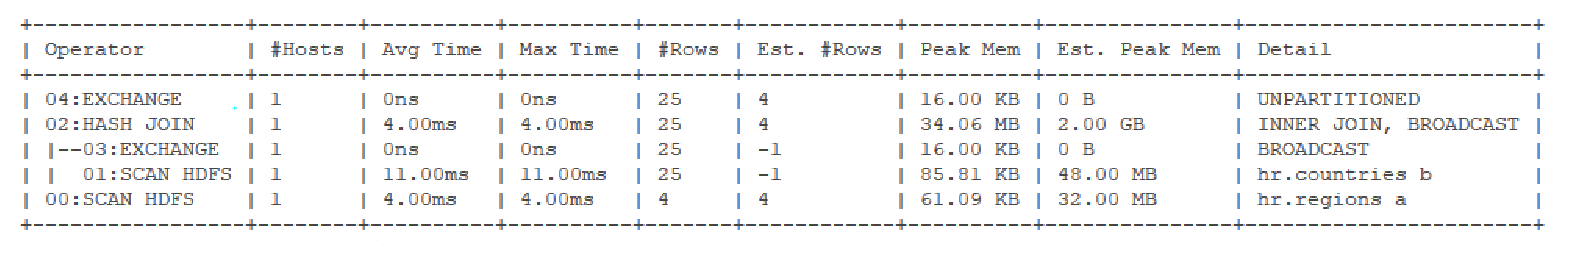
\includegraphics[height=2in, keepaspectratio]{summary.eps}
    \caption{Output of the SUMMARY command for a query.}
    \end{center}
\end{figure}


The PROFILE command produces an extremely detailed account of the execution.
It begins with summary information about the query and the connection that submitted it.
It then provides a detailed look at how the query plan was broken into fragments, and information associated with those fragments.
If any table involved in the query is missing statistics, a warning will appear just above this section naming those tables so that you can choose to update their statistics.
Following the definition of these fragments is an extremely granular look at the execution of each individual fragment. 
It provides information on the time required to produce the first result as well as the full result, along with a large amount of other information about timing, memory usage, and other statistics about the fragment.
It is likely that most of this information will not be useful to you, but it can provide a more granular look at execution times than other commands. 

The Metrics section in the impalad interface contains additional information about the current and past behavior of the impalad. Of particular interest in this section are: 

\begin{itemize}
    \item Boolean indicating connection to statestore
    \item Topic update version numbers
    \item Quantiles for the execution time of queries and DDL
    \item Detailed memory usage for various aspects of the node
\end{itemize}


\section{File Formats}
The choice of data structure is an important decision that influences performance, stability and accessibility.
Tabular data are inherently rectangular.
More strictly, every row has the same set of column nodes and every record share same variables. 
In contrast, columnar storage stores data in columns. 
The database can then access the data more precisely and prevent from scanning the unwanted data in row. 
This structure can efficiently write and read data from storage disk. 
Dremel and Solar are two successful distributed system that implement shared everything architecture with columnar data structure. 
According to the Dremel paper, it claims that columnar- nested data structure help their shared disk system access data faster and reduce CPU cost due to cheaper compression \cite{Dremel}.
On the other hand, Solar used the share everything architecture base on tree data set. 
They increase the performance and scalability by adding storage nodes that are used for data storage and read access \cite{zhu2018solar}.  

Impala supports several file formats that used in Apache Hadoop. 
Impala can also load and query data from different files produced by Pig or Hive. 
It is important to choose file format used in Impala table since file format has significant impacts on the performance.
For example, some file formats enable compression that may affect size of data and consequently lead to I/O and CPU resources required to deserialize data.
With this advantage, it can limit the query performance since querying often involves decompressing data. 
To reduce the data transfer time from disk to memory, compressing data can bring a smaller number of data to being processed. 
Some file formats are structured, which included metadata and built-in compression. 
File formats supported in Impala are: Parquet, Avro, Text, RCFile, and SequenceFile. 
On the other hand, Avro, Parquet and Optimized Row Columnar (ORC) are three optimized file formats that used in Hadoop clusters. 
Each of these file formats are unique and have their own relative advantages and disadvantages.  
        \subsection{Parquet}
Parquet is a column-oriented file format.
In contrast to row-oriented approach, it is more efficient for storage and performance.
The values of each columns are organized and adjacent, so that it enables better compression. 
Since that, Parquet is a good choice when you need to query a specific column with wide table, or work on some aggregation operations such as SUM() and AVG() that need to process most of the values in a column. 
Parquet table can minimize I/O by reading less data and retrieve values from column quickly, and thus improve the performance because the I/O cost may strongly influenced by the number of columns needed to be processed. 
On the other hand, some complex types such as ARRAY, STRUCT and MAP are currently supported only by the Parquet file format. 

When you try to load data that is already in the Impala or Hive table into Parquet table, even if the data is in a different file format or partitioning scheme, you can easily use the Impala INSERT...SELECT syntax.
The block size is the number of segments which hold columns entries in the Parquet file.
For Parquet table, INSERT statement  requires space in the HDFS to write one block, and its default block size is 1 GB.
If the HDFS does not have enough space, an INSERT might fail. When the system fail to INSERT into a partitioned table due to lack of the capacity, you can use hint keyword [SHUFFLE] or [NOSHUFFLE] (including the square brackets) before the SELECT keyword and after the PARTITION clause.
[SHUFFLE] reduces overall resource usage by select the query plan that has the minimized number of files being written into HDFS.
[NOSHUFFLE] may bring to an insertion failure as well because it select a faster query plan and sometime create large number of small data, so it is not recommended. 
Impala will choose use or not to use the hint depends on the number of values in columns and the number of nodes that going to be process in the INSERT operation. 
        \subsection{Avro}
Avro is a row major file format.
Impala can query and create Avro tables, but not insert them. 
For insertion, you can use Hive to accomplish and switch back to Impala. 
LOAD DATA can be used in both Avro and Impala if there already have Avro data file. 
Impala can move it to the Avro table but not create new Avro data file. 
Avro schemas are defined with JSON and so it stores data definition in JSON after creating Avro tables.
Currently, Avro tables does not support TIMESTAMP columns.
There are two functions that help to store time values: UNIX\_TIMESTAMP() or EXTRACT().
UNIX\_TIMESTAMP() convert the STRING type of values into BIGINT type, and EXTRACT() create separate columns for date and time fields.

For some reason, mismatch of values type may occur between Avro schema and column definition in the database.
To solve this problem, Impala uses schema reconciliation to check mismatching number of columns. 
Impala will choose to use the definition in Avro schema when there is mismatch in number of column, column name and column type. 
For the restriction mentioned above, a TIMESTAMP definition in Impala maps to Avro STRING, which is a representation in the Avro schema.
Moreover, Avro supports schema evolution to handle old and new schema. 
Meanwhile, people can work with different version of schema at the same time.

        \subsection{ORC}
Optimized Row Columnar (ORC) stores data in column format.
To be more specific, it stores collections of rows data into a columnar layout.
This enables parallel processing for row collections. 
Each row data is called stripe. 
In a stripe, it contain index data, row data that is used in table scan and stripe footer. 
At the end of the file has file footer and postscript to store some information such as numbers of rows, compression parameter and column-level aggregate min, max, sum and count. 

ORC is an optimized version of RCFile.
It makes improvement on the compression by using an encoder that handle different column data types. 
ORC also skips blocks of rows that are not needed in query and then indexing fewer files and reduce load. 
Same as Avro, ORC does not support INSERT operation. 
You can create ORC tables in Impala, load or insert data through Hive and then query them in Impala.  
Considering mismatch of the data types in ORC table, it has defined sets of types that has different name in Impala format. 
For instances, ORC BINARY to Impala STRING. On the other hands, complex types are not supported. 



\section{Appendix}
	
\nocite{*}
\bibliographystyle{IEEEtran}
\bibliography{references}
    
\end{document}